\documentclass{article}

\usepackage[letterpaper, margin=1in]{geometry}
\usepackage{underscore}
\usepackage{titling}
\usepackage{listings}
\usepackage{amsmath}
\usepackage{titlesec}
\usepackage{enumitem}
\usepackage{booktabs}
\usepackage{color}
\usepackage{xspace}
% \usepackage[normalem]{ulem}

\usepackage[utf8]{inputenc}
\usepackage[pdftex]{graphicx}
\DeclareGraphicsExtensions{.pdf,.png}
\graphicspath{{img/}}


%New colors defined below
\definecolor{codegreen}{rgb}{0,0.6,0}
\definecolor{codegreen}{rgb}{0,0.6,0}
\definecolor{codegray}{rgb}{0.5,0.5,0.5}
\definecolor{codepurple}{rgb}{0.58,0,0.82}
\definecolor{backcolour}{rgb}{0.95, 0.95, 0.95}
\definecolor{darkred}{rgb}{0.9,0,0}
%Code listing style named "mystyle"
\lstdefinestyle{mystyle}{
  % backgroundcolor=\color{backcolour},
  commentstyle=\color{darkred},
  keywordstyle=\color{blue},
  numberstyle=\tiny\color{codegray},
  stringstyle=\color{codegreen},
  basicstyle=\small,
  breakatwhitespace=false,
  breaklines=true,
  captionpos=b,
  keepspaces=true,
  numbers=left,
  numbersep=5pt,
  showspaces=false,
  showstringspaces=false,
  showtabs=false,
  tabsize=4
}
\lstset{language=sql}
\lstset{style=mystyle}

\titleformat{\section}{\Large\bfseries}{}{0em}{}

\titlespacing{\section}{0em}{0.3ex plus 0.1ex minus 0.05ex}{0.1ex plus 0.1ex}
\titlespacing{\subsection}{0em}{0.3ex plus 0.1ex minus 0.05ex}{0.1ex plus 0.1ex}

\renewcommand{\thesubsection}{\arabic{subsection}}
\newcommand{\ze}{she\xspace}

\titleformat{\subsection}{\bfseries}{}{0em}{}

\setlist[enumerate]{topsep=2pt, itemsep=0pt, leftmargin=*}
\setlist[itemize]{topsep=2pt, itemsep=0pt, leftmargin=*}

\setlength{\parskip}{\baselineskip}

\usepackage{indentfirst}

% \usepackage{hyperref}
% \hypersetup{colorlinks=true, urlcolor=blue}
% \urlstyle{same}

\usepackage{cleveref}
\Crefname{figure}{Fig.}{Figs.}

\title{Snickr}
\author{Dov Salomon}


\renewcommand{\maketitle}{
\begin{center}
{\huge\bfseries\thetitle} \\
\vspace{3pt}
{\large\theauthor} \\
\vspace{3pt}
\today
\end{center}
}

\newcommand{\attribs}[1]{\{\texttt{#1}\}}

\setlength{\abovedisplayskip}{0pt}
\setlength{\belowdisplayskip}{0pt}
\setlength{\abovedisplayshortskip}{0pt}
\setlength{\belowdisplayshortskip}{0pt}

\begin{document}

\maketitle

\section{Introduction}

In this report I will describe the database design for a web-based collaboration app \textit{snickr}, which similar to Slack, is comprised of workspaces and channels in which users can communicate. First, I will outline the relational schema and its corresponding ER diagram. I will also give an equivalent database schema for the MySQL DBMS that implements this design. Afterward, I will show example queries on the schema using test data.

\section{Relational Schema}
{
\ttfamily
\noindent
User(\underline{uname}, nickname, email, password) \\
Workspace (\underline{wsname}, description) \\
Wsmember(\underline{wsname}, \underline{uname}, admin) \\
Channel(\underline{chname}, \underline{wsname}, owner, chtype) \\
Chmember(\underline{chname}, \underline{wsname}, \underline{member}) \\
Invitation(\underline{chname}, \underline{wsname}, \underline{invitee}) \\
Message(\underline{msgid}, chname, wsname, sender, content)

\noindent
\textnormal{Foreign Keys:}

\begin{tabular}{lcl}
Wsmember(uname)                 & references & User(uname) \\
Wsmember(wsname)                & references & Workspace(wsname) \\
Channel(wsname, owner)          & references & Wsmember(wsname, uname) \\
Chmember(chname, wsname)        & references & Channel(chname, wsname) \\
Chmember(wsname, owner)         & references & Wsmember(wsname, uname) \\
Invitation(chname, wsname)      & references & Channel(chname, wsname) \\
Invitation(wsname, invitee)     & references & Wsmember(wsname, uname) \\
Message(wsname, chname, sender) & references & Chmember(wsname, chname, member) \\
\end{tabular}
}

For readability (and brevity) I have omitted the timestamp field of each table. (These are included in the schema shown in \Cref{lst:schema}.)

Instead of using a globally unique channel id, each channel is uniquely identified by the tuple (\texttt{chname}, \texttt{wsname}). This allows us to ensure that a user can only be made a member of a channel if \ze is a member of the channel's workspace simply by checking a foreign key constraint.

I chose to make the \texttt{msgid} globally unique, as opposed to only unique in a channel, since it shortens the primary key, and doesn't limit the power of the database to make efficient integrity checks.

Additionally I have chosen to model the direct channel in the same way that the public and private channels are modeled. This will rely on the web application to ensure that direct channels only have 2 members at all times. The name of the direct channel can be some text encoding of the 2 usernames containing characters that are not allowed in regular channel names, which will ensure that the chname is available. This could be achieved more rigorously by using a separate modeling, but would increase the complexity and presents a design tradeoff. I chose this approach because the model stil has enough expressive power, without the added complexity.

\section{ER Diagram}

\Cref{fig:er} shows the ER diagram of the design.

 \begin{figure}[!ht]
 	\centering
 	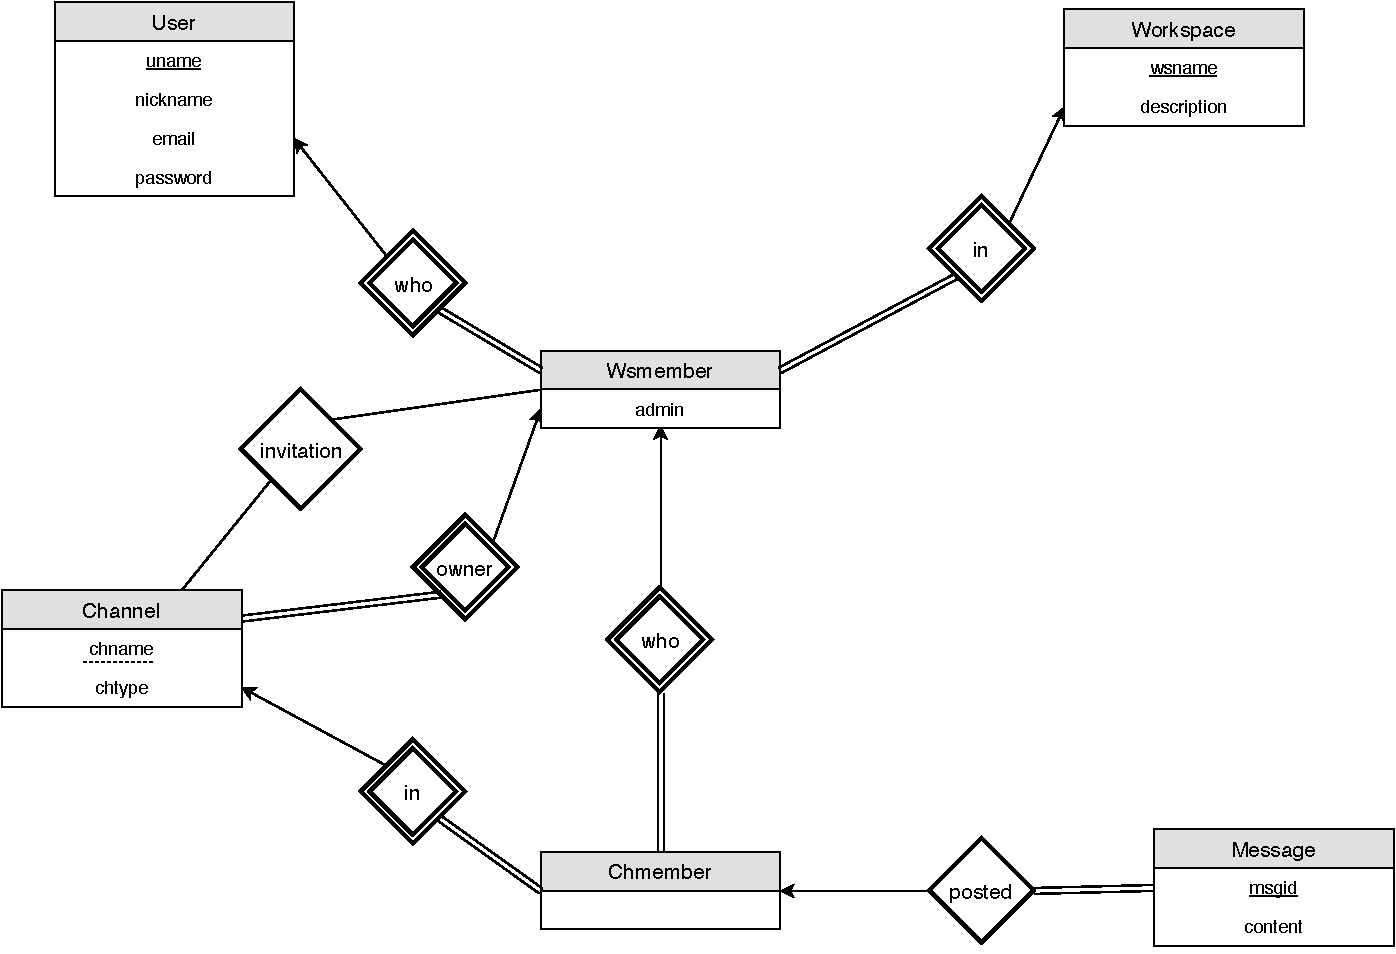
\includegraphics[width=0.9\linewidth]{dber}
 	\caption{The ER diagram.}
 	\label{fig:er}
\end{figure}

There are a few notes to make on this ER diagram. Firstly, while this ER diagram suggests that the primary key for Channel should be (\texttt{uname}, \texttt{wsname}, \texttt{chname}), in reality the primary key is (\texttt{wsname}, \texttt{chname}) since we want to enforce that a channel name is unique to a workspace. That said, the channel table does have a foreign key for (\texttt{uname}, \texttt{wsname}) referencing \texttt{Wsmember} (\texttt{uname}, \texttt{wsname}) since we want to enforce that a user can only create a channel for workspaces that \ze is a member.

\section{MySQL Schema}

\Cref{lst:schema} below shows the MySQL schema for the database design. It follows directly from the Relational Schema.

\lstinputlisting[caption=Database Schema,label=lst:schema]{../sql/schema.sql}

I decided to use \texttt{enum} for the \texttt{chtype} field in the \texttt{channel} table since there are only 3 possible values. It is also more space efficient and performant then using \texttt{varchar}.

I chose varchar(64) as the length for the name fields, but this could be shorter or longer as needed in practice.


\section{Test Dataset}

The test data is shown in \Crefrange{tbl:user}{tbl:message} and consists of 2 workspaces, generically named \textit{job} and \textit{baseball}. There are users that in both workspaces, neither workspace, and in just one of the workspaces. Each channel also has a private and public channel, with some users being in both or neither.


\begin{table}[!p]
\centering
\begin{tabular}{l l l l}
\toprule
\multicolumn{1}{c}{uname} &
\multicolumn{1}{c}{nickname} &
\multicolumn{1}{c}{email} &
\multicolumn{1}{c}{password} \\
\midrule
george  & George    & george@nyu.edu  & password123     \\
john    & John      & john@nyu.edu    & elephant        \\
james   & James     & james@nyu.edu   & password123     \\
har     & Harriet   & har@nyu.edu     & abcdef          \\
sam     & Samantha  & sam@nyu.edu     & ghijkl          \\
dorothy & Dorothy   & dorothy@nyu.edu & password123     \\
trisha  & Patricia  & trish@nyu.edu   & xyz             \\
jen     & Jennifer  & jen@nyu.edu     & lll             \\
\bottomrule
\end{tabular}
\caption{User table.}
\label{tbl:user}
\end{table}

\begin{table}[!p]
\centering
\begin{tabular}{l l}
\toprule
\multicolumn{1}{c}{wsname} &
\multicolumn{1}{c}{description} \\
\midrule
job & Work \\
baseball & Play \\
\bottomrule
\end{tabular}
\caption{Workspace table.}
\label{tbl:ws}
\end{table}

\begin{table}[!p]
\centering
\begin{tabular}{l l l}
\toprule
\multicolumn{1}{c}{wsname} &
\multicolumn{1}{c}{uname} &
\multicolumn{1}{c}{admin} \\
\midrule
job & george  & true   \\
job & john    & false  \\
job & james   & false  \\
job & har     & false  \\
job & sam     & true   \\
\midrule
baseball & george & false \\
baseball & har & false \\
baseball & sam & true \\
baseball & trisha  & true \\
baseball & dorothy & false \\
\bottomrule
\end{tabular}
\caption{Workspace Member table.}
\label{tbl:wsmember}
\end{table}

\begin{table}[!p]
\centering
\begin{tabular}{l l l l}
\toprule
\multicolumn{1}{c}{uname} &
\multicolumn{1}{c}{chname} &
\multicolumn{1}{c}{owner} &
\multicolumn{1}{c}{chtype} \\
\midrule
job & general & george & public \\
job & managers & sam & private \\
\midrule
baseball & general & sam & public \\
baseball & pitchers & har  & private \\
\bottomrule
\end{tabular}
\caption{Channel table.}
\label{tbl:channel}
\end{table}

\begin{table}[!p]
\centering
\begin{tabular}{l l l}
\toprule
\multicolumn{1}{c}{wsname} &
\multicolumn{1}{c}{chname} &
\multicolumn{1}{c}{member} \\
\midrule
job & general & george \\
job & general & john   \\
job & general & james  \\
job & general & har    \\
job & general & sam    \\
\midrule
job & managers & george \\
job & managers & sam   \\
job & managers & har   \\
\midrule
baseball & general & george  \\
baseball & general & har     \\
baseball & general & sam     \\
baseball & general & trisha  \\
\midrule
baseball & pitchers & har \\
baseball & pitchers & trisha \\
\bottomrule
\end{tabular}
\caption{Channel Member table.}
\label{tbl:chmember}
\end{table}

\begin{table}[!p]
\centering
\begin{tabular}{l l l l}
\toprule
\multicolumn{1}{c}{wsname} &
\multicolumn{1}{c}{chname} &
\multicolumn{1}{c}{invitee} &
\multicolumn{1}{c}{invited} \\
\midrule
job & managers & john & 2019-04-14 \\
baseball & pitchers & george & 2019-03-01 \\
baseball & general & dorothy & 2019-02-01 \\
\bottomrule
\end{tabular}
\caption{Invitation table.}
\label{tbl:invitation}
\end{table}

\begin{table}[!p]
\centering
\begin{tabular}{l l l l}
\toprule
\multicolumn{1}{c}{wsname} &
\multicolumn{1}{c}{chname} &
\multicolumn{1}{c}{sender} &
\multicolumn{1}{c}{content} \\
\midrule
job & general & har & When is the staff meeting? \\
job & general & george & In 10 minutes. \\
job & general & sam  & That is perpendicular. \\
\midrule
job & managers & george  & What is happening at the staff meeting? \\
\midrule
baseball & general & sam & When is the game? \\
basenall & general & trisha & Next Sunday! \\
\midrule
baseball & pitchers & trisha & Are you pitching on Sunday? \\
baseball & pitchers & har & I will pitch perpendicular \\
\bottomrule
\end{tabular}
\caption{Message table.}
\label{tbl:message}
\end{table}

\section{Example Queries}

In this section I will implement some basic queries, and show the results for the test dataset.

\begin{enumerate}
\item
Create a new user account, with email, name, nickname, and password.
\begin{lstlisting}
insert into user(email, uname, nickname, password) values
('dsalomon@nyu.edu', 'dms833', 'dov', 'password123');
\end{lstlisting}

\item
Create a new public channel inside a workspace by a particular user.
\begin{lstlisting}
insert into channel(wsname, chname, owner, chtype) values
('job', 'random', 'dms833', 'public');
\end{lstlisting}

The foreign key constraint guarantees that dms833 is a member of the job workspace.

\item
For each workspace, list all current administrators.
\begin{lstlisting}
select wsname, uname
from wsmember
where admin;
\end{lstlisting}
\begin{verbatim}
+----------+--------+
| wsname   | uname  |
+----------+--------+
| baseball | sam    |
| baseball | trisha |
| job      | george |
| job      | sam    |
+----------+--------+
\end{verbatim}

\item
For each public channel in a given workspace, list the number of users that were invited to join the channel more than 5 days ago and that have not yet joined.
\begin{lstlisting}
select chname, invitee
from channel join invitation using(wsname, chname)
where wsname = 'baseball'
and chtype = 'public'
and timestampdiff(day, invited, current_timestamp()) >= 5
and (wsname, chname, invitee) not in (
  select wsname, chname, member
  from chmember
);
\end{lstlisting}

The last part of the where clause is not necessarily needed, assuming that an invitation is automatically removed when the user accepts the invitation and is added to the channel.
\begin{verbatim}
+---------+---------+
| chname  | invitee |
+---------+---------+
| general | dorothy |
+---------+---------+
\end{verbatim}

Note that george is not listed here since he was invited to a public channel in the baseball workspace, not a private one.

\item
For a particular channel, list all messages in chronological order
\begin{lstlisting}
select msgid, content
from message
where wsname = 'job'
and chname = 'general'
order by posted;
\end{lstlisting}
\begin{verbatim}
+-------+----------------------------+
| msgid | content                    |
+-------+----------------------------+
|     1 | When is the staff meeting? |
|     2 | In 10 minutes.             |
|     3 | That is perpendicular      |
+-------+----------------------------+
\end{verbatim}

\item
For a particular user, list all messages they have posted in any channel.
\begin{lstlisting}
select msgid, content, wsname, chname
from message
where sender = 'george';
\end{lstlisting}
\begin{verbatim}
+-------+-----------------------------------------+--------+----------+
| msgid | content                                 | wsname | chname   |
+-------+-----------------------------------------+--------+----------+
|     2 | In 10 minutes.                          | job    | general  |
|     4 | What is happening at the staff meeting? | job    | managers |
+-------+-----------------------------------------+--------+----------+
\end{verbatim}

\item
For a particular, list all messages that are accessible to this user and that contain the keyword “perpendicular” in the body of the message.
\begin{lstlisting}
select msgid, content
from message join chmember using(wsname, chname)
where chmember.member = 'george'
and content like '%perpendicular%';
\end{lstlisting}
\begin{verbatim}
+-------+-----------------------+
| msgid | content               |
+-------+-----------------------+
|     3 | That is perpendicular |
+-------+-----------------------+
\end{verbatim}

We can also try out this query for a few other users.

\begin{lstlisting}
select msgid, content
from message join chmember using(wsname, chname)
where chmember.member = 'trisha'
and content like '%perpendicular%';
\end{lstlisting}
\begin{verbatim}
+-------+----------------------------+
| msgid | content                    |
+-------+----------------------------+
|     8 | I will pitch perpendicular |
+-------+----------------------------+
\end{verbatim}

\begin{lstlisting}
select msgid, content
from message join chmember using(wsname, chname)
where chmember.member = 'har'
and content like '%perpendicular%';
\end{lstlisting}
\begin{verbatim}
+-------+----------------------------+
| msgid | content                    |
+-------+----------------------------+
|     3 | That is perpendicular      |
|     8 | I will pitch perpendicular |
+-------+----------------------------+
\end{verbatim}

The following has no output since dorothy is not in any channels.
\begin{lstlisting}
select msgid, content
from message join chmember using(wsname, chname)
where chmember.member = 'dorothy'
and content like '%perpendicular%';
\end{lstlisting}

\end{enumerate}

\end{document}
